% Template for PLoS
% Version 3.3 June 2016
%
% % % % % % % % % % % % % % % % % % % % % %
%
% -- IMPORTANT NOTE
%
% This template contains comments intended
% to minimize problems and delays during our production
% process. Please follow the template instructions
% whenever possible.
%
% % % % % % % % % % % % % % % % % % % % % % %
%
% Once your paper is accepted for publication,
% PLEASE REMOVE ALL TRACKED CHANGES in this file
% and leave only the final text of your manuscript.
% PLOS recommends the use of latexdiff to track changes during review, as this will help to maintain a clean tex file.
% Visit https://www.ctan.org/pkg/latexdiff?lang=en for info or contact us at latex@plos.org.
%
%
% There are no restrictions on package use within the LaTeX files except that
% no packages listed in the template may be deleted.
%
% Please do not include colors or graphics in the text.
%
% The manuscript LaTeX source should be contained within a single file (do not use \input, \externaldocument, or similar commands).
%
% % % % % % % % % % % % % % % % % % % % % % %
%
% -- FIGURES AND TABLES
%
% Please include tables/figure captions directly after the paragraph where they are first cited in the text.
%
% DO NOT INCLUDE GRAPHICS IN YOUR MANUSCRIPT
% - Figures should be uploaded separately from your manuscript file.
% - Figures generated using LaTeX should be extracted and removed from the PDF before submission.
% - Figures containing multiple panels/subfigures must be combined into one image file before submission.
% For figure citations, please use "Fig" instead of "Figure".
% See http://journals.plos.org/plosone/s/figures for PLOS figure guidelines.
%
% Tables should be cell-based and may not contain:
% - spacing/line breaks within cells to alter layout or alignment
% - do not nest tabular environments (no tabular environments within tabular environments)
% - no graphics or colored text (cell background color/shading OK)
% See http://journals.plos.org/plosone/s/tables for table guidelines.
%
% For tables that exceed the width of the text column, use the adjustwidth environment as illustrated in the example table in text below.
%
% % % % % % % % % % % % % % % % % % % % % % % %
%
% -- EQUATIONS, MATH SYMBOLS, SUBSCRIPTS, AND SUPERSCRIPTS
%
% IMPORTANT
% Below are a few tips to help format your equations and other special characters according to our specifications. For more tips to help reduce the possibility of formatting errors during conversion, please see our LaTeX guidelines at http://journals.plos.org/plosone/s/latex
%
% For inline equations, please be sure to include all portions of an equation in the math environment.  For example, x$^2$ is incorrect; this should be formatted as $x^2$ (or $\mathrm{x}^2$ if the romanized font is desired).
%
% Do not include text that is not math in the math environment. For example, CO2 should be written as CO\textsubscript{2} instead of CO$_2$.
%
% Please add line breaks to long display equations when possible in order to fit size of the column.
%
% For inline equations, please do not include punctuation (commas, etc) within the math environment unless this is part of the equation.
%
% When adding superscript or subscripts outside of brackets/braces, please group using {}.  For example, change "[U(D,E,\gamma)]^2" to "{[U(D,E,\gamma)]}^2".
%
% Do not use \cal for caligraphic font.  Instead, use \mathcal{}
%
% % % % % % % % % % % % % % % % % % % % % % % %
%
% Please contact latex@plos.org with any questions.
%
% % % % % % % % % % % % % % % % % % % % % % % %

\documentclass[10pt,letterpaper]{article}
\usepackage[top=0.85in,left=2.75in,footskip=0.75in]{geometry}

% amsmath and amssymb packages, useful for mathematical formulas and symbols
\usepackage{amsmath,amssymb}

% Use adjustwidth environment to exceed column width (see example table in text)
\usepackage{changepage}

\usepackage{times}

% Use Unicode characters when possible
\usepackage[utf8x]{inputenc}

% textcomp package and marvosym package for additional characters
\usepackage{textcomp,marvosym}

% cite package, to clean up citations in the main text. Do not remove.
\usepackage{cite}

% Use nameref to cite supporting information files (see Supporting Information section for more info)
\usepackage{nameref,hyperref}

% line numbers
\usepackage[right]{lineno}

\usepackage{comment}

% ligatures disabled
\usepackage{microtype}
\DisableLigatures[f]{encoding = *, family = * }

% color can be used to apply background shading to table cells only
\usepackage[table]{xcolor}

% array package and thick rules for tables
\usepackage{array}

% create "+" rule type for thick vertical lines
\newcolumntype{+}{!{\vrule width 2pt}}

% create \thickcline for thick horizontal lines of variable length
\newlength\savedwidth
\newcommand\thickcline[1]{%
  \noalign{\global\savedwidth\arrayrulewidth\global\arrayrulewidth 2pt}%
  \cline{#1}%
  \noalign{\vskip\arrayrulewidth}%
  \noalign{\global\arrayrulewidth\savedwidth}%
}

% \thickhline command for thick horizontal lines that span the table
\newcommand\thickhline{\noalign{\global\savedwidth\arrayrulewidth\global\arrayrulewidth 2pt}%
\hline
\noalign{\global\arrayrulewidth\savedwidth}}


% Remove comment for double spacing
%\usepackage{setspace}
%\doublespacing

% Text layout
%\raggedright
\setlength{\parindent}{0.5cm}
\textwidth 5.25in
\textheight 8.75in

% Bold the 'Figure #' in the caption and separate it from the title/caption with a period
% Captions will be left justified
%\usepackage[aboveskip=1pt,labelfont=bf,labelsep=period,justification=raggedright,singlelinecheck=off]{caption}
\usepackage[aboveskip=1pt,labelfont=bf,labelsep=period,justification=justified,singlelinecheck=off]{caption}
\renewcommand{\figurename}{Fig}

% Use the PLoS provided BiBTeX style
\bibliographystyle{plos2015}

% Remove brackets from numbering in List of References
\makeatletter
\renewcommand{\@biblabel}[1]{\quad#1.}
\makeatother

% Leave date blank
\date{}

% Header and Footer with logo
\usepackage{lastpage,fancyhdr,graphicx}
\usepackage{epstopdf}
\pagestyle{myheadings}
\pagestyle{fancy}
\fancyhf{}
\setlength{\headheight}{27.023pt}
\lhead{
\includegraphics[width=2.0in]{PLOS-submission.eps}}
\rfoot{\thepage/\pageref{LastPage}}
\renewcommand{\footrule}{\hrule height 2pt \vspace{2mm}}
\fancyheadoffset[L]{2.25in}
\fancyfootoffset[L]{2.25in}
\lfoot{\sf PLOS}

%% Include all macros below

\newcommand{\lorem}{{\bf LOREM}}
\newcommand{\ipsum}{{\bf IPSUM}}

\usepackage{afterpage}

%% END MACROS SECTION

\begin{document}
\vspace*{0.2in}

% Title must be 250 characters or less.
% Please capitalize all terms in the title except conjunctions, prepositions, and articles.
\begin{flushleft}
{\Large
\textbf\newline{%Self-organised criticality in a Boolean Network Model of the Evolution of Cortical Development}
%A Baldwin Effect in a Boolean Network Model of the Evolution of Cortical Development}
Modelling the Evolution of Cortical Development: A Baldwin Effect}
}
\newline
% Insert author names, affiliations and corresponding author email (do not include titles, positions, or degrees).
\\
Stuart P. Wilson\textsuperscript{1,2*}, Daniel Whiteley\textsuperscript{1,2}, Sebastian S. James,\textsuperscript{1,2}, Leah A. Krubitzer\textsuperscript{3}
\\
\bigskip
\bf{1} Department of Psychology, The University of Sheffield, Sheffield, United Kingdom,\\
\bf{2} Sheffield Robotics, The University of Sheffield, Sheffield, United Kingdom,\\
\bf{3} Center for Neuroscience, University of California, Davis, California 95618, United States.
\bigskip

% Use the asterisk to denote corresponding authorship and provide email address in note below.
* S.P.Wilson@sheffield.ac.uk

\end{flushleft}

% Please keep the abstract below 300 words
\section*{Abstract}

How can the developmental dynamics of network self-organisation constrain the evolutionary dynamics of natural selection? We address this fundamental question in the specific context of the gene-interaction networks that shape neocortical development, and ask how self-organisation within such networks might constrain the search for genes that help establish functional cortical maps. At embryonic day 8 (E8), the morphogen fibroblast growth factor 8 (Fgf8) is expressed in mice only in the anterior pole of the developing forebrain \cite{Sur2005,Rakic2009}. Later in development Emx2, Pax6, Coup-tf1, Sp8, and other genes are expressed as gradients that configure the anterior-posterior axis of the neocortex and, in part, construct the sensory and motor areas that ultimately compose the neocortex\cite{Greig2013}. Assuming for simplicity that gene expression levels are binary, the interactions between these five genes can be modelled using a Boolean network, with the `genome' for a 5-gene network comprising $80$ binary variables, and the space of possible genomes thus comprising $2^{80}$ possibilities. Randomly sampling this space yields an estimate that by chance 1-2 genomes in 100,000 will specify a network that from the E8 expression pattern will eventually settle into the mature pattern of gradients. The problem can be formulated as one in which the corresponding initial and final states, i.e., gene expression patterns, should occupy two attractors (anterior versus posterior) in the network dynamics. Accordingly, we show that a relationship between the genome configuration and the emergent attractor landscape can be exploited by a simple evolutionary algorithm, such that successful networks can be discovered at a rate much greater than chance. The emergent evolutionary dynamics resemble `punctuated equilibria', and the distribution of discovery rates conforms to an exponential relationship. Importantly, this interaction between self-organisation (within lifetime) and selection (between lifetimes) emerges in the model without any direct exchange of information from phenotype to genotype. The model is therefore discussed in terms of the Baldwin effect.

% Please keep the Author Summary between 150 and 200 words
% Use first person. PLOS ONE authors please skip this step.
% Author Summary not valid for PLOS ONE submissions.
\section*{Author Summary}

Self-organisation and natural selection are two fundamental forces that shape all biological systems. Self-organisation typically describes developmental dynamics that unfold within the lifetime of an individual organism, whereby ordered biological patterns emerge spontaneously from unordered initial conditions. The laws that govern self-organisation are thought by some to constrain the nature of the adaptations to the environment that may in principle be discovered by natural selection. Progress towards exposing such theories to empirical testing can be made by identifying a specific biological network in which the interactions can be manipulated directly. To this end, we model self-organising interactions between the genes whose expression patterns are known to affect the division of the cortex into distinct visual, auditory, somatosensory, and motor areas. We then simulate the evolution of this gene network using a simple evolutionary algorithm, and show that this algorithm can exploit structure in the relationship between the genotype and the self-organising phenotype to more rapidly discover successful gene networks. The model therefore shows how the nature of self-organising dynamics may influence the course of natural selection, to discover specific gene networks whose interactions in developing mammal brains ultimately influence cortical organisation, connectional networks, and information processing.


\linenumbers

\section*{Introduction}

As the mammalian brain develops, the functional organisation of the neocortex emerges from a complex interaction between genetic and environmental influences (see \cite{Krubitzer2018} for review). For the processing of primary sensory and motor information, the mature cortex is functionally specialised into localised regions that respond primarily to input from specific sensor arrays, such as the retinae, the cochleae, and the skin, muscles and joints. The arealization of the cortex into corresponding primary visual, primary auditory, and primary somatosensory areas, as well as into secondary sensory areas and motor and pre-motor areas, emerges from both activity-dependent competitive interactions between thalamocortical axons as they grow into the cortex prenatally, and from sensory-driven processes that continue as the animal matures \cite{REFS}. A basic schematic for the arealization pattern of the mature cortex is established early in the embryonic development of the forebrain by a set of gradients in the expression levels of transcription factors which specify position information in the cortex and ultimately guide the growth of thalamocortical axons (e.g., \cite{Sur2005,Ypsilanti2016}; see \cite{Greig2013,Anton2018} for review). The target of natural selection is the adaptive sensory mediated behaviour that the neocortex generates. However, in shaping the functional organisation of the cortex, selection has been reconfiguring the gene-interaction networks that specify the chemoattractive gradients involved in cortical arealization. In this study, we ask how the developmental dynamics within gene-interaction networks responsible for guiding the process of cortical arealization may constrain the evolution of cortical maps. %In this context, computational modelling is a useful methodology for revealing the laws of complexity in general terms, as well as for testing intuitions about specific complex systems in our natural world \cite{}.%, and for revealing the laws of complexity in more general terms \cite{}.

The anterior telencephalic morphogen Fgf8 \cite{Shimogori2005}, and the transcription factors Emx2, Pax6, Coup-tf1, and Sp8 are an important subset of the genes known to substantially impact the patterning of the neocortex during early prenatal development (e.g., \cite{Hamasaki2004,Manuel2007,Borello2014,Armentano2007,Greig2013}). For example, Emx2 knockout mice display an anterioly shifted primary somatosensory region \cite{Bishop2000,Bishop2002}, and ectopic expression of Fgf8 can cause duplication of the primary sensory areas \cite{Assimacopoulos2012}. In wild type mice, the expression level of four of these genes comes to define a gradient with respect to an anterior to posterior axis through the forebrain (Fig.\,1). For Pax6, and Sp8, the gradient that develops is from high expression levels in the anterior region to low expression levels in the posterior region. For Emx2 and Coup-tf1 the gradient is reversed from low to high in the anterior/posterior axis.

At embryonic day 9.5, before the other transcription factors are known to be expressed, Fgf8 (as well as other signalling molecules and patterning centers) is secreted only at the anterior neural ridge of the developing forebrain (\cite{Rakic2009}; see \cite{Greig2013} for review). Together with other signalling centers, the secretion of Fgf8 at embryonic day 9.5 induces the graded expression of Emx2, Pax6, Coup-tf1, and Sp8 in the progenitor cells in the ventricular zone. However the precise network of interactions between these genes has not yet been fully characterised. To better understand the network of gene interactions responsible for cortical patterning, Giacomantonio and Goodhill (2010, \cite{Giacomantonio2010}) considered the expression level of each gene at the anterior and the posterior position as a binary occurrence (e.g., Pax6 is expressed at the posterior location or it is not). They then conceptualised the potential interactions between genes in terms of a set of Boolean logic operations, with each pattern of the gene expression triggering either the activation or inactivation of each of the other genes, leading to a cascade of interactions that represents the embryonic development of the forebrain.

Giacomantonio and Goodhill defined a set of constraints on how the networks should be constructed based on available evidence from previous experiments with mice, and then used a computer to iterate through the developmental dynamics of the large number of networks that satisfy these constraints, in order to identify the features of such networks from which the observed gradients reliably emerge. For example, the interaction between Sp8 and Fgf8 was fixed to be excitatory in all simulated networks because this interaction had been experimentally established in mice \cite{Sahara2007}.

Adding such constraints vastly reduced the search space for candidate networks. Hence, the purpose of the original investigation was to systematically explore the remaining unknown aspects of this mouse gene-interaction network, and to suggest how gaps in the experimental evidence relating to these interactions in an extant species (mouse) might be filled based on  common properties of successful simulated networks. Here we use a similar computational approach to interrogate the same network of five interacting genes, but we ask an importantly different question: In the space of all \emph{possible} interactions between five genes, how common are networks that lead from an initial high expression level in one gene at one of two locations, to the observed pattern of opposing gradients between all five genes? Assuming that the robust emergence of opposing gradients in extant species indicates a selective advantage to the emergence of such gradients, we then ask how likely are such networks to have been discovered by natural selection? Finally, we ask whether any potential relationship between the structure of the genome space in which gene-interaction networks evolve, and the structure of the phenotype space in which gene interactions develop, may in principle constrain the evolution of cortical development.

%We assume that because this developmental pattern is robustly observed in extant mammals, any gene-interaction network that supports it should be considered favourable to natural selection. In these terms we can deconstruct the central question into the following. How numerous are these `fit’ networks in the entire space of possible networks in which natural selection has been operating? Might more general structural commonalities amongst fit networks be revealed by considering regions of this space beyond that which correspond to extant species? In principle, might any such structure have be exploited by natural selection in the discovery of fit networks?

\section*{Models}

If we describe the expression level of a gene as being either high ($1$) or low ($0$), then the pattern of gene expression levels produced by a network of $n$ interacting genes may at any instance adopt one of $2^n$ possible states. As the genes interact with one another their relative expression levels will change, and thus the network will transition through a series of states. We can model the interactions that give rise to these state transitions using the Boolean networks formalism \cite{Kauffman1993}. Accordingly, transitioning from one network state to the next requires evaluating for each gene the expression levels of the $n-1$ other genes. Thus, associated with each gene is a truth table which specifies whether each of the $2^{n-1}$ possible combinations of `input' registered by that gene will cause its `output' expression level to next be $1$ or $0$. Specifying the output for every possible combination of inputs, for all genes in the network,  requires a `genome' of $N=n2^{n-1}$ binary variables. Hence the space of possible gene interaction networks is of size $2^N$, which corresponds to the number of possible genomes. In this $2^N$-- dimensional `binary genome space', we are interested in those genomes that specify the developmental dynamics observed in mice, wherein differential expression of one gene (Fgf8) leads to a cascade of gene interactions that results in the emergence of a persistent pattern of opposing expression gradients (see Fig.~1). %We will later be representing evolution by natural selection as a directed walk through genome space.

\vspace{1em}\emph{\noindent Please insert Figure 1 about here.}\vspace{1em}

Specifically, a Boolean network of $n=5$ genes, representing Fgf8, Emx2, Pax6, Coup-tf1, and Sp8, with expression levels correspondingly labelled $a$--$e$, should transition from an `initial anterior state' in which $a=1$ and $b=c=d=e=0$ to an `anterior mature state' in which $a=c=e=1$ and $b=d=0$, and it should transition from a `posterior initial state' in which $a=b=c=d=e=0$ to a `posterior mature state' in which $a=c=e=0$ and $b=d=1$. As a short-hand, we can write the initial anterior, initial posterior, mature anterior, and mature posterior states as binary sequences $10000$, $00000$, $10101$, and $01010$, or we can translate these sequences into integers
% decimals not integers? SJ
 and refer simply to states $16$, $0$, $21$, and $10$. As such, we are interested in genomes that specify gene-interaction networks in which state $16$ leads eventually to state $21$, as in the mouse anterior forebrain, and in which state $0$ leads eventually to state $10$, as in the mouse posterior forebrain.

%Iterative application of the Boolean interactions that are specified by a given genome creates a dynamic pattern of binary expression levels that in the present model represents the early genetic interactions that occur during embryonic development of the forebrain.
Activation dynamics in Boolean networks self-organise to reveal attractors, such that from a number of initial states the network will eventually settle into cycling through a particular sequence of states endlessly. This set of repeating states is known as the limit cycle. An attractor comprises the set of states from which a given limit cycle will be reached, and amongst the $2^n$ possible states of the network one or more attractors may emerge. In the case where the limit cycle comprises only one (repeating) state the attractor is referred to as a point attractor. The attractors of a network can be found by iterating its dynamics from each initial state $s$ until any state is revisited, and the number of iterations before any state is revisited in this process (minus the number of states in the limit cycle) provides a measure of the distance $d_s$ of that initial state from the limit cycle.

In the present model, we assume that once the pattern of gene expression gradients emerges, it should remain stable and persistent, at least until the basic cortical arealization pattern has been established. This translates to the assertion i) that states $21$ and $10$ should be the only states occupying the limit cycles of two point attractors in the network dynamics. From this assertion it follows ii) that states $16$ and $21$ should occupy the same attractor, iii) that states $0$ and $10$ should occupy the same attractor, and iv) that the attractors occupied by these two pairs of states should be different.

By these criteria we may define a `maximally fit genome' ($f=1$) as one whose developmental dynamics satisfy criteria i, ii, iii, and iv. We may also define any genome whose developmental dynamics do not satisfy these four criteria as being less fit ($0\leq f<1$). As such, we can explore the fitness landscape in the genome space by generating many genomes, establishing the attractor landscape in the network dynamics specified by each, and measuring the extent to which they satisfy criteria i--iv. The proportion of maximally fit genomes discovered in this process can be used to define a baseline discovery rate.

To ask whether any potential structure to the embedding of the gene networks in the genome space may be exploited by natural selection to discover maximally fit genomes, an initially random genome can be iteratively modified, with only modifications that improve fitness surviving into subsequent generations. The rate at which fit networks are discovered by this simple evolutionary process can then be compared to the baseline discovery rate. Two crucial points are important to emphasise here. Firstly, it is important to emphasise that this evolutionary procedure should involve no direct transmission of information about the state of the phenotype (the emergent pattern of gene expression), to the genome that is survived into subsequent generations. Secondly, such an evolutionary procedure can therefore only be expected to improve the rate at which maximally fit networks are discovered if there is a pre-existing systematic relationship between the genotype and the phenotype, i.e., if proximal genomes yield comparable attractor dynamics. We hypothesise that such a relationship does exist, insofar as an appropriate fitness function may be defined in order to guide evolution to more rapidly discover networks in which complementary gene expression gradients develop.

\section*{Results}

Triggered by the differential expression of one gene (Fgf8) in the anterior versus posterior forebrain, a cascade of interactions between (at least) five genes results in the development of a stable set of opposing anterior-posterior gene expression gradients. Considering the expression levels of these genes as binary, at each of two locations (anterior and posterior), and the interactions between these genes as Boolean logic operations, we first establish the rate at which networks displaying such dynamics should be expected to be discovered by chance, i.e., the proportion of such networks occupying the `genome space'. We then show that there is a structure to the embedding of these network specifications into the genome space, and that this structure can be used to guide a simple evolutionary process to discover fit genomes at a higher rate.

All figures in this paper can be recreated using the source code available in the supplementary materials as \emph{S1 Code}.

\subsection*{A `needle in a haystack' problem}

First we consider a simple network of $n=3$ interacting genes. In this example, the binary genome space comprises $2^N=4,096$ Boolean networks (where $N=n2^{n-1}$), and the analogous problem can be formulated as one in which initial states (i.e., gene expression patterns) $100$ and $000$ should lead to corresponding mature states $101$ and $010$ as the only states occupying the limit cycles of two distinct attractors. An exhaustive search revealed that no genomes satisfy these criteria, and hence for networks of $n=3$ genes the problem is insoluble (see Supplementary Figure S2 for an explanation).

Next we consider networks of $n=4$ genes and the corresponding genome space which comprises $2^{32}=4,294,967,296$ possible genomes. In this case the problem is to find networks where the initial anterior state $1000$ and the initial posterior state $0000$ lead to the corresponding target states $1010$ and $0101$. Knowing that in such networks iterating the target states $1010$ and $0101$ must transition directly to those same two states again allows a motif of $2n=8$ of the 32 variables in the genome to be set, and thus the genome space can be exhaustively searched by mapping out the attractor landscapes of only $2^{32-8}=16,777,216$ candidate networks. An exhaustive search of this genome (sub-) space identified $475,122$ successful networks, i.e., 0.011\%.

For $n=5$ genes there are $2^{80}$ possible genomes. The goal is to find networks where initial states 16 ($10000$) and 0 ($00000$) lead to the corresponding target states 21 ($10101$) and 10 ($01010$) as the only states occupying the limit cycle of separate attractors. Fig.~2 shows the attractor landscape in one example of a maximally fit network of $n=5$ interacting genes. Knowing that iterating the target states $10101$ and $01010$ must lead directly to those two states again allows a motif of $2n=10$ of the 80 variables in the genome to be set, and thus for the attractor landscapes of only $2^{70}$ networks to be mapped out by iterating their dynamics in full. Nonetheless an exhaustive search is not feasible. Instead we generated $2^{32}$ random genomes (for comparison with the $n=4$ case), and discovered $59,088$ maximally fit networks, i.e., 0.0014\%. Therefore, we estimate that the baseline rate at which maximally fit networks should be discovered by blind search for networks of $n=5$ genes is between 1 and 2 in every $100,000$ generations.

\vspace{1em}\emph{\noindent Please insert Figure 2 about here.}\vspace{1em}

Together these simulation results indicate that the problem of developing opposing gene expression patterns may be solved for networks comprising a minimum of $n=4$ genes, and that this `needle-in-a-haystack' problem increases in complexity as the number of interacting genes increases.

\subsection*{Evolution of cortical development}

Instead of searching the genome space randomly, we can modify our definition of fitness to also favour genomes that do not necessarily specify maximally fit networks, but which display some of the properties of maximally fit networks, and then iteratively mutate the genome, accepting only mutations that increase fitness. To this end, we define a fitness function that favours also networks ($n=5$) which from the initial states 16 and 0 occupy the corresponding target states 21 and 10 \emph{at some later stage} in the developmental dynamics, with a fitness that increases for target states that are fewer iterations from the limit cycles. Specifically, if conditions ii, iii, and iv are met (see \emph{Models}), and $d_s$ is the distance of state $s$ from the limit cycle, then the fitness of the genome, $f$, is defined as,

\begin{equation}
f=1-\left(d_{10}+d_{21}\right)/2^{n+1},
\end{equation}

\noindent or else $f=0$. To simulate evolution in this model, we maintain a single genome, and in each generation flip each binary variable with a fixed probability $p\in\{0,0.5\}$, and survive the modified genome into the next generation only if the fitness was increased as a result ($\Delta f>0$).

This simple evolutionary procedure was iterated for a total of ten million generations at each of three mutation rates ($p=0.3$, $p=0.35$, $p=0.4$), with a new random genome generated following the discovery of each maximally fit network ($f=1$). The resulting evolutionary dynamics are displayed in Fig.~3, which shows the discovery of ten maximally fit networks. The evolution reveals a dynamics similar to `punctuated equilibria', in which increasingly long periods of stasis ($\Delta f=0$) are punctuated by increments in fitness \cite{Gould1977,Bak1996}.

\vspace{1em}\emph{\noindent Please insert Figure 3 about here.}\vspace{1em}

The number of maximally fit networks that were discovered in this way, as a proportion of the number of generations simulated, was more than double the baseline discovery rate of $1.4\times 10^{-5}$ previously established: $3.4\times 10^{-5}$ for $p=0.3$, $3.8\times 10^{-5}$ for $p=0.35$, and $3.1\times 10^{-5}$ for $p=0.4$. %of 0.0014\% previously established: 0.0034\% for $p=0.3$, 0.0038\% for $p=0.35$, and 0.0031\% for $p=0.4$. %Thus, selecting for point attractors with states at the limit cycle that are closer (smaller Hamming distance) from the target states reveals a smoothness to the distribution of fit genomes in genome space that can be exploited to accelerate their discovery by natural selection.
Histograms, $y(x)$, constructed for the number of generations taken to discover maximally fit genomes ($x$) in Fig.~4 reveal that discovery rates are distributed according to an exponential relationship. Curves fitted by linear regression to the model $\log y(x)=\alpha x+\beta$ yield similar estimates of the exponent at each mutation rate: $\alpha=-3.23\times 10^{-5}$ for $p=0.3$,  $\alpha=-3.86\times 10^{-5}$ for $p=0.35$, and $\alpha=-2.70\times 10^{-5}$ for $p=0.4$. %, with exponents X for $p=0.3$, Y for $p=0.35$, and Z for $p=0.4$.

\vspace{1em}\emph{\noindent Please insert Figure 4 about here.}\vspace{1em}

These results together confirm our hypothesis that the genotype (the specification of Boolean network interactions) and the phenotype (the emergent attractor dynamics) are related in a way that can be exploited to accelerate the evolutionary search  without direct transmission of information from phenotype to genotype between generations. This indicates that developmental attractor landscapes are embedded within the genome space according to some non-random structure, i.e., nearby genomes specify gene-interaction networks that yield similar attractor dynamics.

\subsection*{Smoothing the fitness landscape}

To visualise the fitness landscape, two approaches were taken. First we computed the average fitness at each generation across all maximally fit genomes discovered, after re-aligning the evolutionary trajectories in each case to the generation at which the maximally fit network was discovered. A profile of fitness rising towards the fitness peaks obtained by this method suggests that the fitness increases approximately exponentially, in a manner that is robust to the mutation rate $p$ as the only free parameter of the model (Supplementary Figure S3). However, the portrait of the fitness landscape revealed by averaging in this way is difficult to reconcile with the punctuated equilibria seen in individual evolutionary trajectories, and may be misleading as a potential artefact of averaging over evolutionary trajectories that increase rapidly from zero to non-zero fitness at intervals distributed exponentially. Therefore we also profiled the fitness landscape by measuring the reduction in fitness after successive mutations of a sample of maximally fit genomes, by looking at \emph{all} genomes at a given Hamming distance (number of mutations) from these fitness peaks. Fig.~5 suggests that the proportion of networks with non-zero fitness (i.e., those in which the initial and complementary mature expression patterns correctly occupy distinct attractors) decreases approximately exponentially with the number of mutations $m$ of the maximally fit genome.

\vspace{1em}\emph{\noindent Please insert Fig.~5 about here.}\vspace{1em}

This decrease is what might be expected if a constant number of variables in the genome, $k$, define a specific motif that must be present in order for fitness to be non-zero. For example, we have already noted that specification of $2n$ specific variables is required if the two target states are to transition into themselves indefinitely. Genomes with positive fitness less than 1 need not contain this particular $2n$ motif, but if they are genomes that do not mutate $k$ immutable variables, then the number of genomes with non-zero fitness should be ${{N-k}\choose{m}}$ out of a total ${{N}\choose{m}}$ possible genomes at $m$ mutations from a maximally fit genome, or

\begin{equation}
h(m,k)=\frac{(N-k)! (N-m)!}{N!(N-k-m)!}.
\end{equation}

This function correctly predicts an approximately exponential decrease in the proportion of genomes with non-zero fitness as a maximally fit genome is mutated (i.e., it can be rewritten as a combination of gamma functions), and provides a good approximation to the empirically derived proportions shown in Fig.~5, assuming $k\approx 14$ for networks of $n=4$ genes (i.e., a motif of 14 out of 32, or 44\%, immutable variables), and assuming $k\approx 26$ for networks of $n=5$ genes (i.e., an ensemble of 26 out of 80, or 33\%, immutable variables). However, by inspection we could find no such fixed motif amongst genomes with fitness $0<f<1$. Therefore we conclude that networks with non-zero fitness are specified by an ensemble of boolean \emph{interactions}, the complexity of which is determined by the relationship between a constant number of binary variables.

%We therefore accept this ensemble hypothesis, and suggest that the particular smoothness of the fitness landscape around the fitness peaks reflects a significant genetic redundancy in the specification of the required developmental dynamics.


%This decrease discriminates clearly between two subtly different hypotheses. According to the first, a constant number of variables in the genome, $k$, define a specific motif that cannot be mutated without causing fitness to be zero. For example, we have already noted that specification of $2n$ specific variables is required if the two target states are to transition into themselves indefinitely. Hence the genomes with non-zero fitness could be those which \emph{do not} mutate these immutable variables. Accordingly, the proportion of genomes with non-zero fitness would be $h_0(m)=1-{{k}\choose{m}}/{{N}\choose{m}}$. However the hypothesis represented by $h_0$ predicts an \emph{increase} in the proportion of genomes with non-zero fitness with each mutation, and we could identify no such motif from the distribution of variables amongst genomes of non-zero fitness, hence we reject this motif hypothesis.

%An alternative hypothesis is that an `ensemble' of variables, of constant size $k$, are redundant insofar as they can be mutated without causing fitness to be zero. The number of genomes with non-zero fitness therefore corresponds to the permutations of this  ensemble of redundant variables. Accordingly, the proportion of genomes with non-zero fitness is predicted to be

%\begin{equation}
%h(m)=\frac{k!(N-m)!}{N!(k-m)!}.
%\end{equation}

%This function correctly predicts an approximately exponential decrease in the proportion of genomes with non-zero fitness (i.e., it can be rewritten as a combination of gamma functions), and provides a good approximation to the empirically derived proportions shown in Fig.~5, assuming $k\approx18$ for networks of $n=4$ genes (i.e., an ensemble of 18 out of 32, or 56\%, redundant variables), and assuming $k\approx55$ for networks of $n=5$ genes (i.e., an ensemble of 55 out of 80, or 69\%, redundant variables). We therefore accept this ensemble hypothesis, and suggest that the particular smoothness of the fitness landscape around the fitness peaks reflects a significant genetic redundancy in the specification of the required developmental dynamics.

Fig.~6 confirms that the average fitness for genomes with non-zero fitness decreases linearly with the number of mutations, which allows the evolutionary search to progress incrementally towards peak fitness. Together these results confirm an approximately exponential portrait of the fitness landscape on the approach to the fitness peaks.

\vspace{1em}\emph{\noindent Please insert Figure 6 about here.}\vspace{1em}

Overall the results demonstrate that while fitness peaks are sparsely distributed in the genome space, an increasing proportion of genomes with non-zero fitness define pathways toward the fitness peaks that can be exploited by a directed random walk in order to find those peaks more quickly. Thus, the model reveals how an inherent relationship between the self-organising developmental dynamics that are specified by similar genotypes, may, in principle, guide the dynamics of evolution by natural selection.

These findings are robust to variations in our definition of maximal fitness, as well as to variations in our definition of non-zero fitness. The fitness function defined by Equation 1 favours only networks that develop correctly with respect to the cortical space, but relaxes the selection pressure with respect to developmental timing, i.e., genomes with $0<f<1$ specify networks that present the target gene-expression pattern, but which do not then continue to do so. In additional simulations we found that comparable results could also be obtained by relaxing selection pressure with respect to space rather than time, by declaring all networks in which the two initial states do not occupy \emph{point} attractors as having zero fitness, and otherwise decreasing fitness linearly with the Hamming distance between the single states occupying the two limit cycles and the corresponding target states (discovery rate $3.02\times 10^{-5}$; $n=5$, $p=0.35$). Note also that re-running the main simulations for two \emph{randomly} selected mature target states, rather than states 10 and 21, yields comparable results, e.g., a discovery rate of $3.21\times 10^{-5}$ ($n=5$, $p=0.35$).% compared to a baseline discovery rate of $1.42 \times 10^{-5}$.

%These findings are robust to variations in our definition of maximal fitness, as well as to variations in our definition of non-zero fitness. The fitness function defined by Equation 1 favours only networks that develop correctly with respect to the cortical space, but relaxes the selection pressure with respect to developmental timing, i.e., genomes with $0<f<1$ specify networks that present the target gene-expression pattern, but which do not then continue to do so. In additional simulations we found that comparable results could also be obtained by relaxing selection pressure with respect to space rather than time, by declaring all networks in which the initial and corresponding mature states do not occupy separate \emph{point} attractors as having zero fitness, and otherwise decreasing fitness linearly with the Hamming distance between the single states occupying the two limit cycles and the corresponding target states (\textbf{data not shown - Dan to confirm}). Note also that re-running the main simulations for two \emph{randomly} selected mature target states, rather than states 10 and 21, yields comparable results, e.g., a discovery rate of $3.21\times 10^{-5}$ ($n=5$, $p=0.35$) compared to a baseline discovery rate of $1.42 \times 10^{-5}$.

%$\beta_4=0.760494919605$, $\beta_5=0.546181315648$, $\alpha_4=0.900663350755$, $\alpha_5=0.962063377159$


\section*{Discussion}

%In the space of all possible (Boolean) interactions between a network of five genes, we first set out to establish the proportion and relationship between those which from the differential expression of one gene lead to the stable emergence of five complementary expression gradients, as occurs in the embryonic mouse forebrain. We then asked whether the genetic specifications for networks that display similar developmental dynamics were related in such a way that the relationship may constrain natural selection.

% We also tried an alternative fitness function.

%

%we define all genomes that specify networks in which the initial anterior and posterior states do not belong to different point attractors as having zero fitness ($f=0$). For the remaining genomes, we measure the Hamming distance of the single state occupying the limit cycle of the attractor that comprises the posterior state 16 from the posterior target state 21 as $h_p$ and the distance of the single state occupying the limit cycle of the attractor that comprises the anterior state 0 from the posterior target state 10 as $h_a$, and define,

%\begin{equation}
%f=1-\alpha(h_p+h_a),
%\end{equation}

%\noindent where $\alpha$ specifies a small (arbitrary) cost to final (stable) gene expression patterns that increases with the deviation of these patterns from the target pattern, and which selection may thus optimise. The rationale is that a gene interaction network that transitions into final states more similar to the full set of complementary expression gradients, while not maximally fit, may nonetheless result in some developmental functionality.


Using a simple evolutionary model, we mapped out the fitness landscape for networks of genes whose expression levels were considered to be binary, and whose interactions were assumed to be Boolean, at the minimal spatial resolution required to specify opposing gradients. Even by this highly simplified analogy, the space of possible networks is considerably vast, and populated sparsely with genomes specifying networks in which the developmental dynamics observed in mice self-organise. However, assuming a relaxed selection pressure, which favours networks whose dynamics establish the emergence of opposing gradients at \emph{any} stage of embryonic development, the fitness landscape was found to be smooth in a way that could be exploited to discover genomes specifying these developmental dynamics at more than double the rate expected by chance. The model therefore shows how, in principle, the intrinsic properties of network self-organisation may impose structures on fitness landscapes that can guide evolution by natural selection. As well as profiling the possible fitness landscape traversed in the evolution of genes Fgf8, Emx2, Pax6, Coup-tf1, and Sp8, which play an important role in cortical patterning, the model shows how self-organisation in gene networks may contribute in more general terms to the emergence of a Baldwin effect.

%% LEAH COMMENT: Need to Discuss here the Greig paper I sent you.

The Baldwin effect refers to the idea that lifetime adaptation can guide and accelerate evolution by natural selection \cite{Baldwin1896}. Baldwin's idea was distinct from Lamarckian evolution, whereby phenotypic adaptations are supposed to be directly inherited. Instead, the Baldwin effect describes a situation where the interaction of the genome with its environment during the lifetime increases the likelihood that the organism will reproduce, such that genes coding for better interactions with the environment will tend to be inherited. The key difference between Lamarckian and Baldwinian evolution is that by the former an adaptation to the environment may be directly inherited, whereas by the latter what is inherited is not the phenotypic adaptation itself but the genetic starting conditions from which the adaptation is more likely to emerge by interaction with the environment \cite{Weber2003}.

%% LEAH COMMENT: I WOULD PROBABLY ADD A PARAGRAPH HERE THAT IS MORE SPECIFIC -  AND REVISE THE PARAGRAPH ABOVE.   1.	Not Lamarckian because you are not inheriting a phenotype. 2.	Inheriting the ability to have a flexible phenotype that allows the brain to match the environment in which it develops. 3.	Genes involved in cellular mechanisms which allows sensory driven activity to construct brain networks (axon guidance, synapse etc..). 4.	Epigenetic mechanisms that affect when and where downstream genes are expressed/transcribed


It is important to recognise that while this environmental interaction is often conceptualised in terms of learning, in fundamental terms the Baldwin effect can be driven by \emph{any} form of ontogenetic adaptation that emerges from the interaction of the genetic information with the extrinsic environment, without a direct Lamarckian exchange of information from phenotype to genotype. This broader perspective is emphasised by Daniel Dennett and others; ``\ldots learning is just a particular case (not in any other way special) of ontogenetic adaptation. The continuity between learning and other purported varieties of self-redesign is taken as given\ldots'' \cite{Dennett2003}. In the present model the interaction with the extrinsic environment is represented, in a minimal sense, by the constraint that the fitness of the genome depends on the specification of different gene expression patterns in each of two distinct environmental contexts, i.e., at the anterior versus the posterior poles of the developing forebrain, where these environmental contexts are represented in the model by the two distinct initial states $10000$ and $00000$ (corresponding to the extrinsically triggered differential expression of morphogen Fgf8 at embryonic day 9.5).

A mechanistic description of the Baldwin effect is provided by Hinton and Nowlan \cite{Hinton1987}. Their seminal paper reports the results of simulations with an evolutionary algorithm tasked with finding a single state of peak fitness in a landscape of $2^{20}$ binary states where all others have zero fitness. They showed that this nearly impossible needle-in-a-haystack task could be solved in just a few hundred generations if a proportion of the genome could be randomly flipped to represent within-lifetime adaptation. The binary state of these adaptable bits could not be directly inherited, but if the fitness decreased with the number of lifetime `flips' required to reach the target, then genomes with more correct non-adaptable bits could be preferentially selected. Hence, the search space was effectively divided into a smaller sub-space in which search for the target configuration of the non-adaptable bits is random, and a second sub-space in which lifetime flipping might then discover the target configuration of the adaptable bits.

The present model gives rise to a Baldwin effect in similar terms, i.e., an undirected search in a subset of the genome space, for non-zero fitness in the vicinity of the fitness peaks, which is subsequently completed by a guided ascent to peak fitness. However, it extends this account by representing ontogenetic adaptation explicitly via a process of network self-organisation, and in doing so supports the view of Dennett by demonstrating that the intrinsic properties of other `varieties of self-redesign' can smooth the fitness landscape in the way that learning alone is otherwise typically assumed to.

Beyond these considerations, the five interacting genes that are represented by our Boolean genome indeed play a central role in the development of the cortical machinery that facilitates the adaptation to the environment that occurs during learning. In this broader context, the present model is a step towards the use of Hebbian models of cortical learning, and specifically of cortical map self-organisation (\cite{Wilson2015,Bednar2016}; an idea considered also by Hinton \& Nowlan), to ask also how the statistics of the animal's environment and the genetically specified chemoattractive gradients interact to shape the evolution of cortical development \cite{Krubitzer2013}. In this regard, a mechanistic model of cortical arealization that explicitly represents the dynamics of both the developing cortical plan and the underlying gene interaction network provides an essential link between models of these processes that have been constructed at different levels of abstraction \cite{Karbowski2004}.

The present model demonstrates how self-organisation and selection might interact in the cortex in terms of embryonic development. It is interesting to note that the intrinsic properties of self-organisation have already been shown to shape the evolution of cortical maps in terms of postnatal development too. Wolf (2005; \cite{Wolf2005}) modelled the postnatal development of topological maps for orientation preference in primary visual cortex using a self-organising (reaction-diffusion) model in which Hebbian-like interactions are strongest between cortical cells that are nearby and also strongest for cells with similar tuning for visual orientation. This model predicts that orientation preference maps resembling those measured in primate primary visual cortex will emerge if interactions based on the physical distances between cells, rather than on their orientation differences, are allowed to dominate the self-organising dynamics. As the weighting of orientation difference in stabilising the dynamics is increased towards the weighting given to physical distance, maps are predicted to emerge in which the density of `pinwheel' singularities converges to $\pi$ (in units of the typical spacing of iso-orientation domains). This remarkable prediction was confirmed in a range of extant species whose lineages diverged in the cretaceous period \cite{Kaschube2010}, evidencing a convergent evolution that has been directed by the intrinsic dynamical properties of map self-organisation by reaction-diffusion. On this basis the authors concluded that ``\ldots the principles of dynamical network self-organization may design and constrain system behaviour as powerfully as an organism's genetic endowment or early life experiences.''.

In the present context of self-organising interactions within the genetic networks that guide cortical arealization, we here arrive at the same conclusion.


%``\ldots my point has always been to stress that learning is just a particular case (not in any other way special) of ontogenetic adaptation. The continuity between learning and other purported varieties of self-redesign is taken as given in the circles in which I converse; learning is adaptive, functional change of one's cognitive (or control) mechanisms, as contrasted with one's digestive mechanisms, reproductive mechanisms, and so on. Hence no part of my purpose was to propose any sort of threshold distinguishing learning as a distinct phenomenon.'' (Dennet, 2003) (Godfrey-Smith, chap. 3, this volume, follows the same familiar policy when he says he is "going to use 'learning' as a short-hand for all facultative mechanisms for acquiring traits.”)” (Dennet, 2003).


%Interpretations of the results of Hinton and Nowlan’s (1987) simulations have been criticised from several angles. However this model still yields the most fundamental demonstration of the potentially powerful effects of lifetime adaptation on evolution by natural selection that were considered by Baldwin. A particularly convincing feature of this demonstration is that the representation of lifetime learning as random bit flipping means that there is no direct communication about the location of the target in the search space between learnable and unlearnable bits. But this is difficult to reconcile with Baldwin's idea of ontogenetic adaptation, that genomes should interact with their environments to generate phenotype candidates for natural selection.

%An instructive example of how the dynamics of self-organisation on developmental timescales may constrain selection on evolutionary timescales is provided by a later aspect of the emergence of cortical maps than considered here. Wolf (2005; \cite{Wolf2005}) modelled the emergence of topological maps for orientation preference in primary visual cortex using a type of reaction-diffusion model in which interactions between cells across the cortical sheet were strongest for cells that are nearby and also strongest for cells with similar orientation preferences. The model predicts that orientation preference maps resembling those measured in primate primary visual cortex will emerge if interactions based on the physical distances between cells, rather than on their orientation differences, are allowed to dominate in stabilising the dynamics of pattern formation, but to a minimal extent. Specifically, as the weighting of orientation difference on the stabilising dynamics is increased towards being equal with the weighting of physical distances, the model predicts that maps will emerge in which the density of pinwheel centers should converge to the constant $\pi$, in `hypercolumn' units defined by the peak in the power of the two-dimensional Fourier transform of the map (i.e., relative to the typical spacing of adjacent iso-orientation domains). Remarkably, this prediction was confirmed in species (tree shrews and galagos, and notably not in rodents) whose common ancestor dates back as the cretaceous period \cite{Kaschube2010}, leading the authors. The prediction of $\pi$-pinwheel density is also found in detailed mechanistic models of sensory-driven map self-organisation in which presentation of natural image stimuli drives Hebbian learning in cortical cells that interact via plastic short-range excitatory and  long-range inhibitory interactions (\cite{Stevens2013}; see \cite{Wilson2016} for a review). Thus, at the level of topological feature maps within a cortical area (V1), the self-organising dynamics of pattern formation that are exploited when continuous maps develop postnatally, contribute at least in equal part to genetic and experience-dependent constrains in shaping the functional organisation of the cortex.



%To summarise, the main results are as follows 1) a minimum of four interacting genes is required to specify network dynamics from which complementary gradients emerge; 2) the evolution of gene-network interactions for $n=5$ genes is a `needle in a haystack’ problem, and for $n>3$, the problem increases; 3) selecting for point attractors with states at the limit cycle that are closer (smaller Hamming distance) from the target states reveals a smoothness to the distribution of fit genomes in genome space that can be exploited to accelerate their discovery by natural selection; 4) Specifically, fit genomes are distributed in the genomes space according to some characteristic distance, as indicated by a peak in the distribution of discovery rates by evolving under this fitness function; 5) relaxing the selection pressure that only point attractors have non-zero fitness reveals an evolutionary dynamics that resembles punctuated equilibria, and a distribution of fit genomes that has a scale-free, self-similar geometry that may be exploited to further accelerate their discovery by natural selection. This is evidenced by the emergence of a power law distribution in the discovery rate; 6) The power law distribution of discovery rates under F2 is robust to the free parameter of the model, the mutation rate $p$, which is a hallmark of self-organised criticality; 7) A non-integer dimension obtained from power law fits to the distribution of discovery rates suggest that the underlying geometry of the fitness landscape under F2 may be fractal.



%%%%%%%%


%%%%%%%%

%The Baldwin Effect is the very powerful idea that lifetime adaptation can speed up the rate of evolution. It is distinct from Lamarckian evolution, whereby phenotypic adaptations are supposed to be directly inherited. Instead, the Baldwin effect describes a situation where the interaction of the genome with its environment during the lifetime increases the likelihood that the organism will reproduce, such that genes coding for better interactions with the environment will tend to be inherited. The key difference between Lamarckian and Baldwinian evolution is that by the former an adaptation to the environment may be directly inherited, whereas by the latter what is inherited is not the phenotypic adaptation itself but the genotypic starting conditions for interactions with the environment that generate adaptive phenotypic forms.



%Interpretations of the results of Hinton and Nowlan’s (1987) simulations have been criticised from several angles. However this model still yields the most fundamental demonstration of the potentially powerful effects of lifetime adaptation on evolution by natural selection that were considered by Baldwin. A particularly convincing feature of this demonstration is that the representation of lifetime learning as random bit flipping means that there is no direct communication about the location of the target in the search space between learnable and unlearnable bits. But this is difficult to reconcile with Baldwin's idea of ontogenetic adaptation, that genomes should interact with their environments to generate phenotype candidates for natural selection.

%We are therefore interested in extending Hinton and Nowlan’s (1987) description of the Baldwin effect, such that the genome of an organism represents only the initial conditions for an interaction with the environment that may (or may not) lead to more highly adapted phenotypes. Such a model would allow us to explore the influence that different properties of the environment might have on the rate of evo- lution towards a target phenotype, and hence to probe the Baldwin effect in more detail. We therefore seek a Hinton-Nowlan–style model that represents ontogenetic adaptation to a (parametric) environment explicitly


\section*{Acknowledgements}

The authors are grateful to Hannes Saal and Jim Stone at the University of Sheffield UK for useful discussions and comments on earlier drafts of the paper.

%If you are reading this at my request, I intend to acknowledge you!

\nolinenumbers

\bibliography{Wilson2018bibfile}

%%%%%%%
\begin{comment}

\begin{thebibliography}{10}

\bibitem{Kauffman1993}
Kauffman SA (1993) The origins of order: {S}elf-organization and selection in
  evolution.
\newblock Oxford University Press.

\end{thebibliography}
\end{comment}
%%%%%%%

%%%%%%%%%%%%%%%%%%%
\newpage
\appendix


\afterpage{
\begin{figure}
\begin{center}
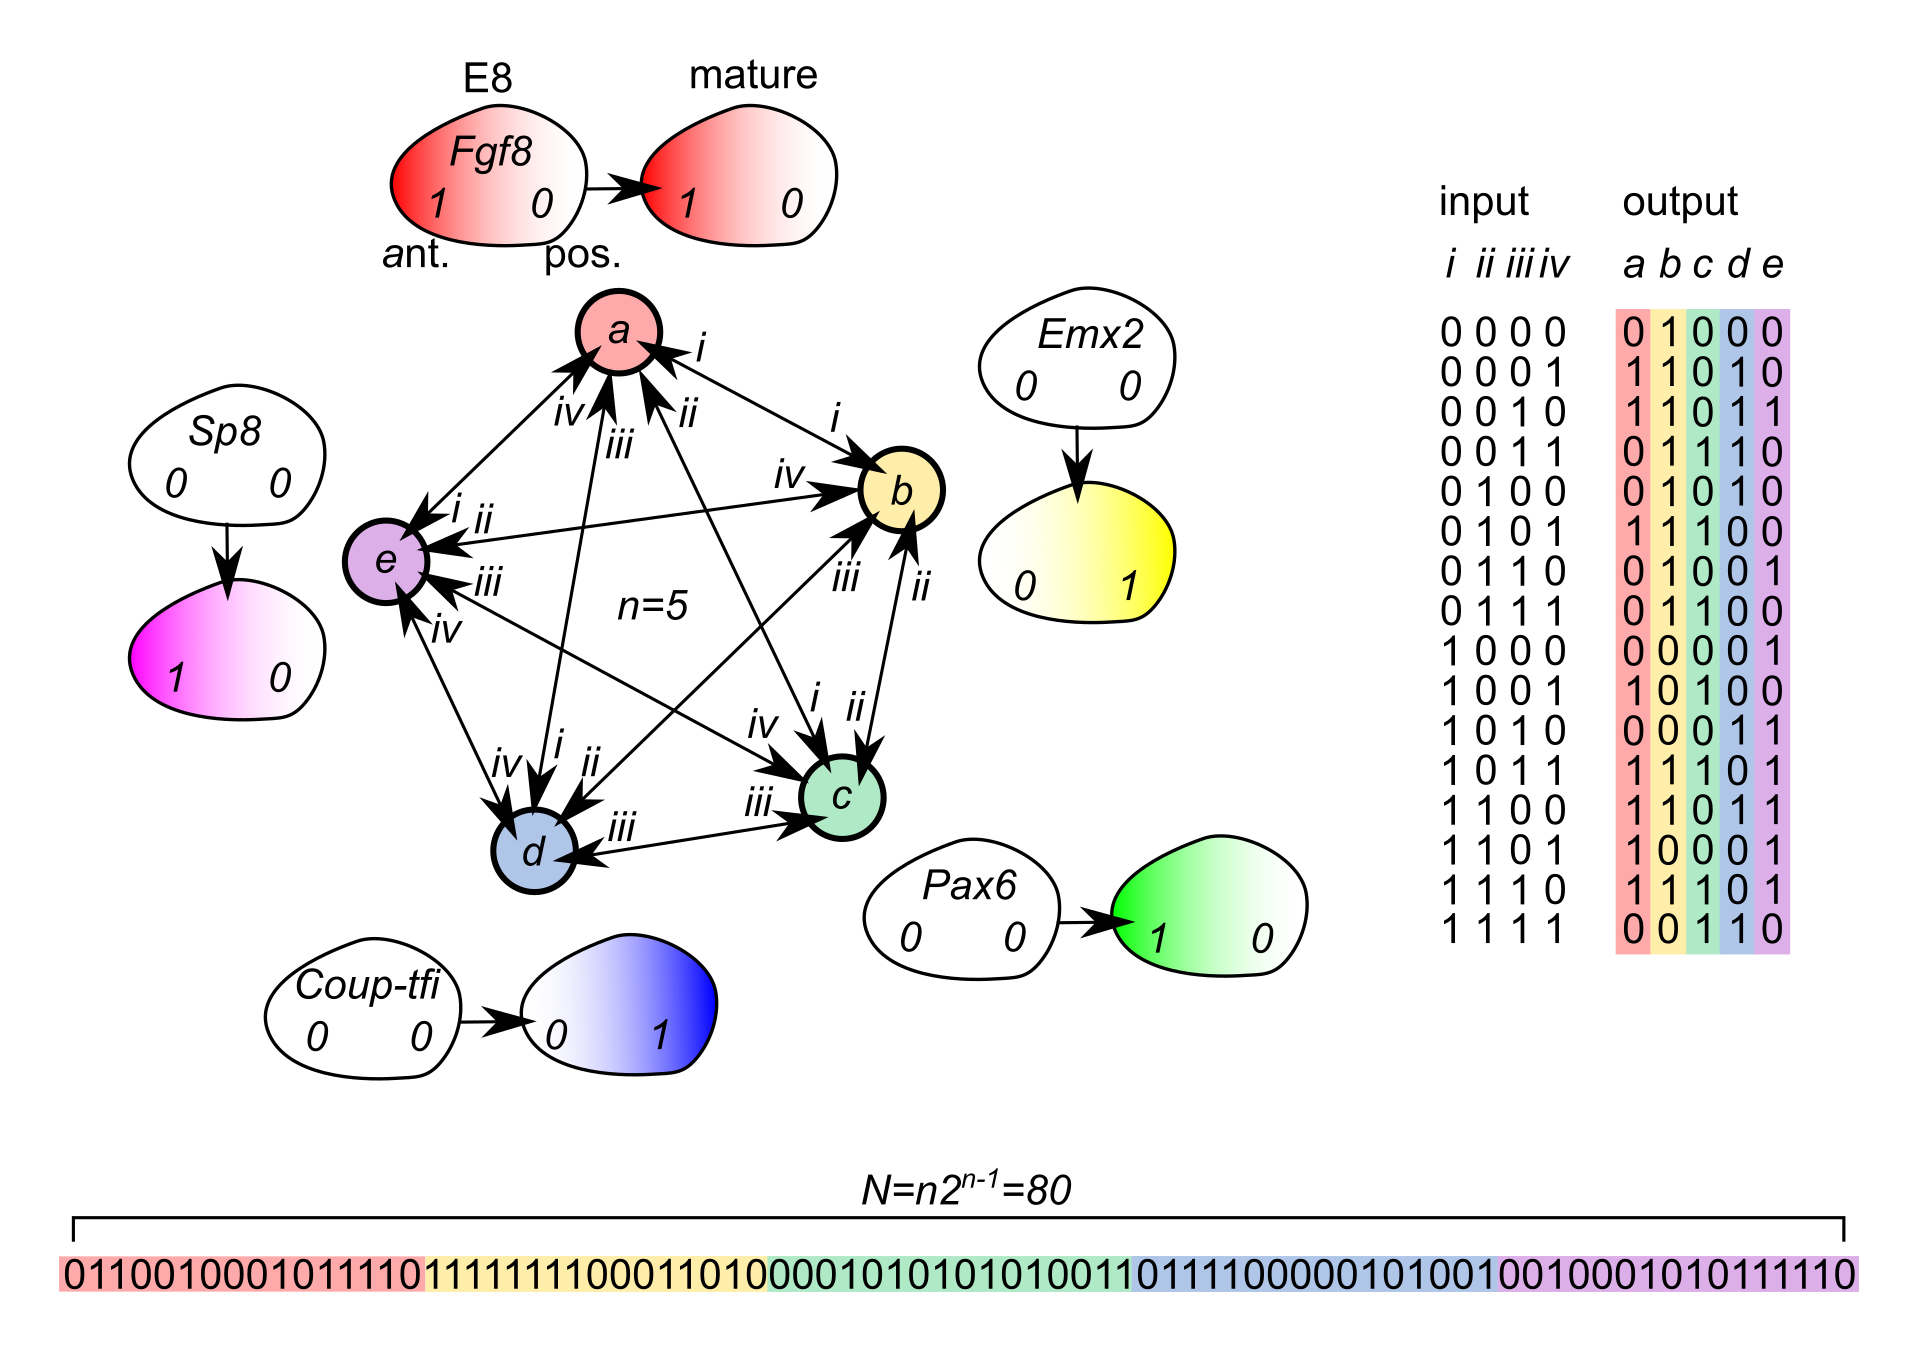
\includegraphics[width=1.0\textwidth,clip=true,trim=0cm 0cm 0cm 0cm]{Figures/Fig1.png}
\caption{\emph{Modelling cortical
    development}. A network of $n=5$ interacting genes are shown
  labelled $a$--$e$. These correspond to genes Fgf8, Emx2, Pax6,
  Coup-tf1, and Sp8. For each gene a schematic depicting the E8 gene
  expression pattern observed in the forebrain of mice at embryonic
  day E8 is shown (with only Fgf8 expressed in only the anterior), as
  well as the direction of the gradient in the expression of each that
  develops with respect to the anterior--posterior axis. In this
  model,  development is represented by the dynamics of a Boolean
  network, with the `output' expression level of each gene affected by
  the pattern of $n-1$ `input' expression levels from the other genes,
  here labelled i--iv. The table on the right specifies, for each of
  $2^{n-1}=16$ possible input patterns, what the output of each gene
  will be, i.e., the expression level on the next iteration of the
  dynamics. The $N=n2^{n-1}=80$ coloured elements of the table are
  thus the binary variables that constitute the genome for this
  network, reproduced as a one-dimensional bit-string below. The
  particular genome specified here is one of $2^N$ possibilities, and
  for illustration purposes is chosen to correspond to a maximally fit
  genome.}
\label{fig:modelling}
\end{center}
\end{figure}
\clearpage}

\afterpage{
\begin{figure}
\begin{center}
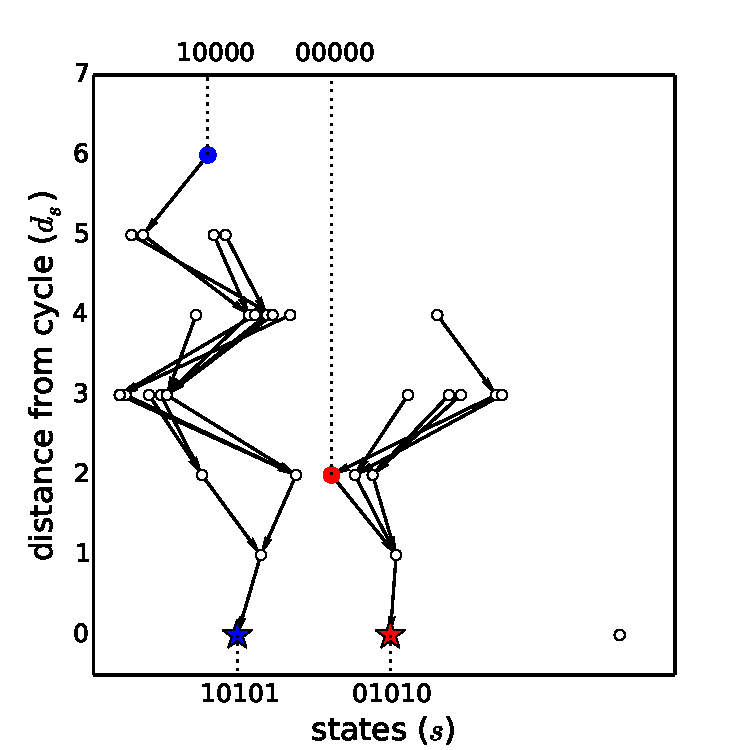
\includegraphics[width=0.7\textwidth,clip=true,trim=0cm 0cm 0cm
  0cm]{Figures/Fig2.pdf}\caption{\emph{Development of a Boolean
    network model of cortical gene-network interactions}. State
  transition diagram for a network of $n=5$ genes that successfully
  maps the initial gene expression levels in the anterior (blue dot)
  and posterior (red dot) to the corresponding target expression
  levels in anterior (blue star) and posterior (red star) after
  several iterations of the gene-network dynamics. Each point is a
  state (a configuration of binary expression levels for $n=5$ genes)
  and all $2^n$ states are shown. Lines connect states that are
  separated by one iteration of the Boolean operations specified by
  this particular genome. States $s$ are ordered on the y-axis by the
  number of transitions that occur before the limit cycle is reached,
  $d_s$, hence states that are further from the limit cycle transition
  into states that are closer to the limit cycle, development proceeds
  through states at incrementally smaller distances from the limit
  cycle, and states at a distance of 0 correspond to point
  attractors. States are separated on the x-axis into three attractors
  (the right-most point is an attractor comprising a single state),
  and within each attractor the states are ordered (arbitrarily) by
  increasing binary index. This particular network is considered
  maximally fit, because the initial states $10000$ and $00000$ map to
  corresponding mature states $10101$ and $01010$ as the only states
  occupying the limit cycle of separate point attractors. Between 1
  and 2 in every 100,000 possible networks is estimated to satisfy
  these criteria.}
\label{fig:development_boolean}
\end{center}
\end{figure}
\clearpage}

\afterpage{
\begin{figure}
\begin{center}
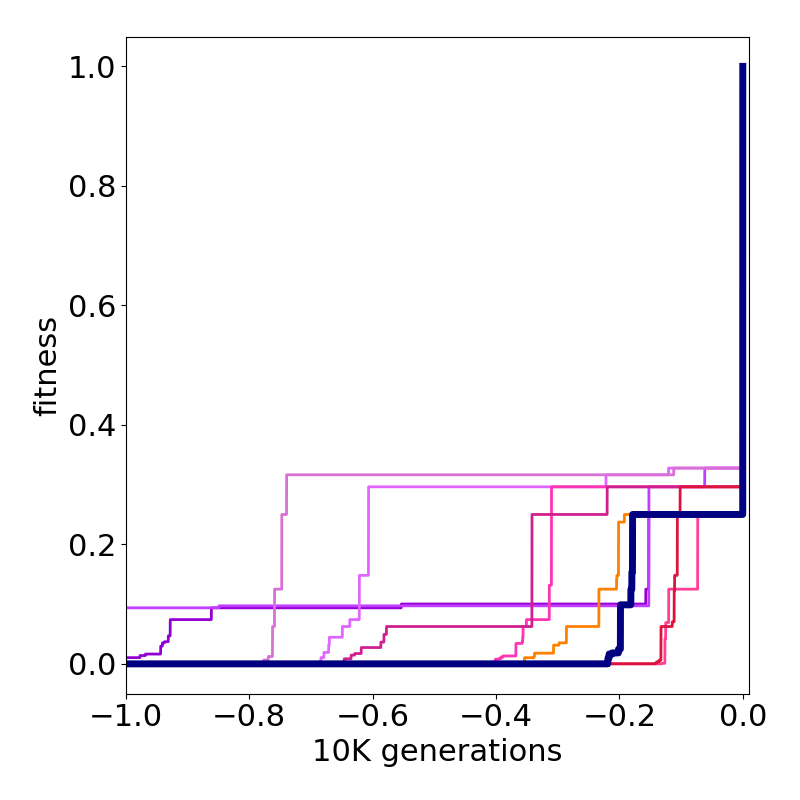
\includegraphics[width=0.7\textwidth,clip=true,trim=0cm 0cm 0cm 0cm]{../simsj/plot/evolution_boolean_ff4.png}
\caption{\emph{Evolution
    of a Boolean network model of cortical gene-network
    interactions}. The discovery of ten maximally fit genomes is
  shown. According to the fitness function (Equation 1), a genome has
  non-zero fitness if proceeding from the initial states $10000$ and
  $00000$ at some point reaches corresponding target states $10101$
  and $01010$ on different attractors, and fitness increases as the
  combined distance of the two target mature states from the limit
  cycle decreases. Traces are aligned so that the generations at which
  maximally fit genomes (fitness $f=1$) are first discovered are
  plotted at generation zero on the right hand side. Evolution in each
  case proceeds from left to right. The characteristic shape of each
  trace indicates that evolution in this model is predicted to proceed
  via long periods of stasis that are punctuated by sharp increases in
  fitness. Thus the evolutionary dynamics predicted by this model may
  be described as `punctuated equilibria'. The trace highlighted with
  a thicker line shows the evolution of the maximally fit network
  whose developmental interactions are represented in Figure 2.}
\label{fig:evolution_boolean}
\end{center}
\end{figure}
\clearpage}


\afterpage{
\begin{figure}
\begin{center}
  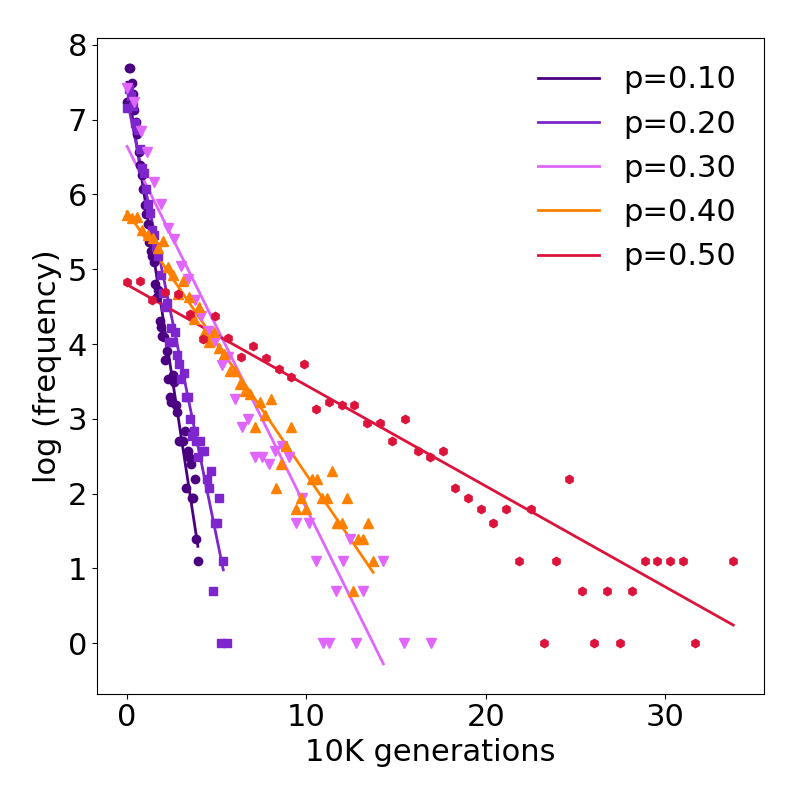
\includegraphics[width=0.7\textwidth,clip=true,trim=0cm 0cm 0cm 0cm]{../simsj/plot/distribution_evolutionary_histo_ff4.png}
  \caption{\emph{Distribution of evolutionary periods between the
      discovery of maximally fit networks}. The evolution of networks
    was continued for a total of 100,000,000 generations. Each time a
    maximally fit network was discovered the genome was randomised and
    the number of generations between the discovery of maximally fit
    networks was recorded. Here we plot the log of the histogram (with
    50 bins) of the number of generations taken to evolve $f=1$
    networks. The process was repeated for mutation rates between
    $p=0.05$ and $p=0.50$, and in each case the logarithmic
    distribution was well approximated by a straight line, indicating
    an exponential relationship. The slope of the fit varied
    approximately linearly over most of the range of mutation rates
    shown (see Fig.~\ref{fig:distribution_evolutionary_slope_vs_p}).}
  \label{fig:distribution_evolutionary_histo}
\end{center}
\end{figure}
\clearpage}

\afterpage{
\begin{figure}
\begin{center}
  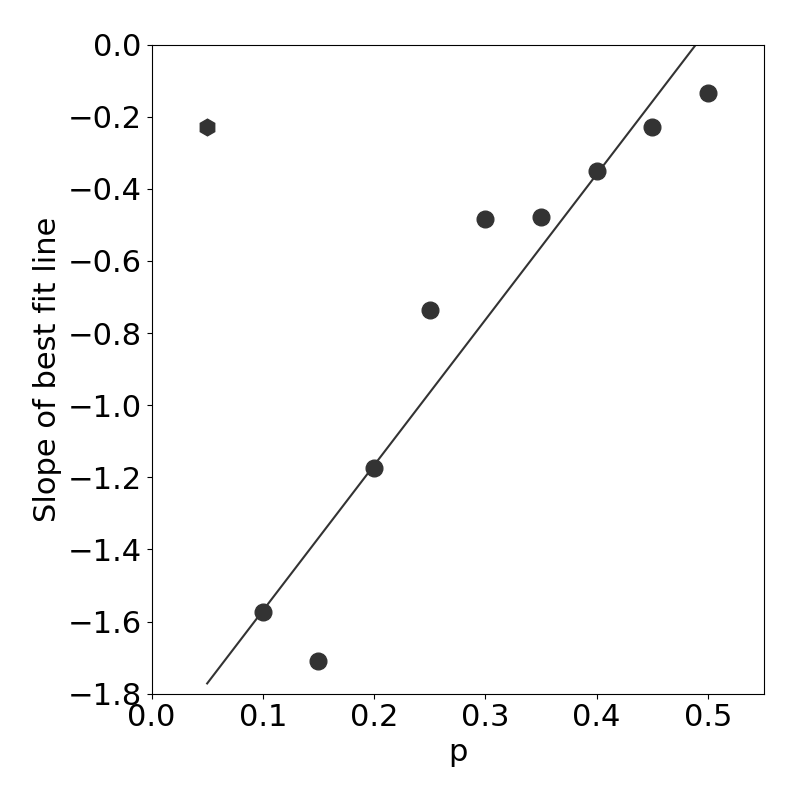
\includegraphics[width=0.7\textwidth,clip=true,trim=0cm 0cm 0cm 0cm]{../simsj/plot/distribution_evolutionary_slope_vs_p_ff4.png}
  \caption{ \emph{The rate of evolution is dependent on the rate of
      mutation}.  The slopes of the linear fits shown in
    Fig.~\ref{fig:distribution_evolutionary_histo} are plotted vs.~the
    mutation rate, $p$, which is the probability of flipping each bit
    of the genome when evolving from one generation to the
    next. Larger and more negative slopes indicate faster evolution
    and so it can be seen that the rate of evolution increases
    approximately linearly with increasing $p$. However, the evolution
    rate must return to zero for $p=0$ and this tendency is seen as
    $p\rightarrow 0$. The hexagonal point for $p=0.05$ was excluded when
    creating the black linear fit line.}
  \label{fig:distribution_evolutionary_slope_vs_p}
\end{center}
\end{figure}
\clearpage}

\afterpage{
\begin{figure}
\begin{center}
  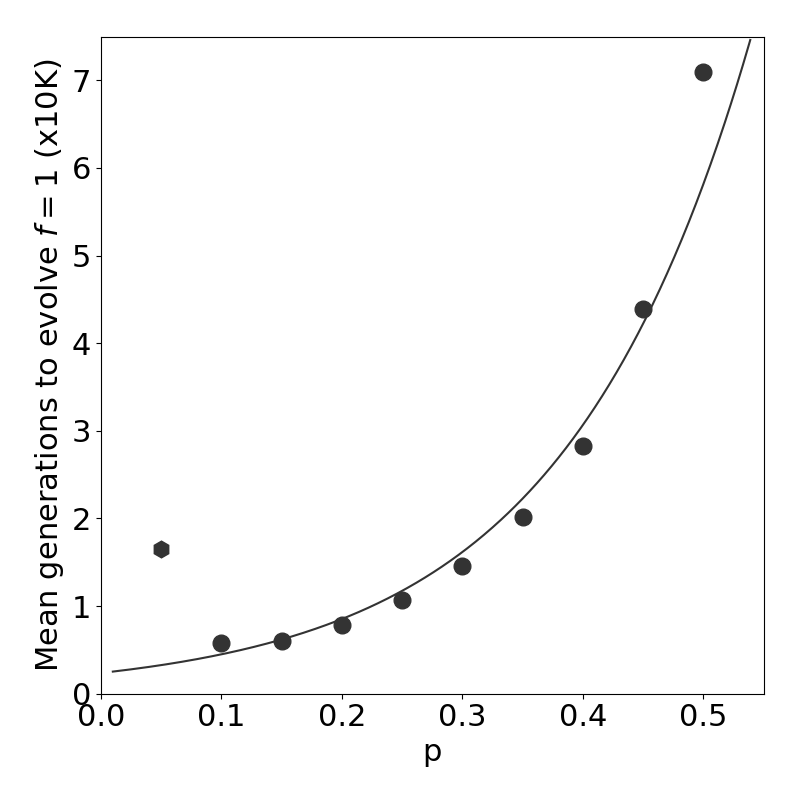
\includegraphics[width=0.7\textwidth,clip=true,trim=0cm 0cm 0cm 0cm]{../simsj/plot/distribution_evolutionary_mean_vs_p_ff4.png}
\caption{\emph{Mean
    number of evolutionary periods between the discovery of maximally
    fit networks} Add extended description.}
\label{fig:distribution_evolutionary_mean_vs_p}
\end{center}
\end{figure}
\clearpage}


\afterpage{
\begin{figure}
\begin{center}
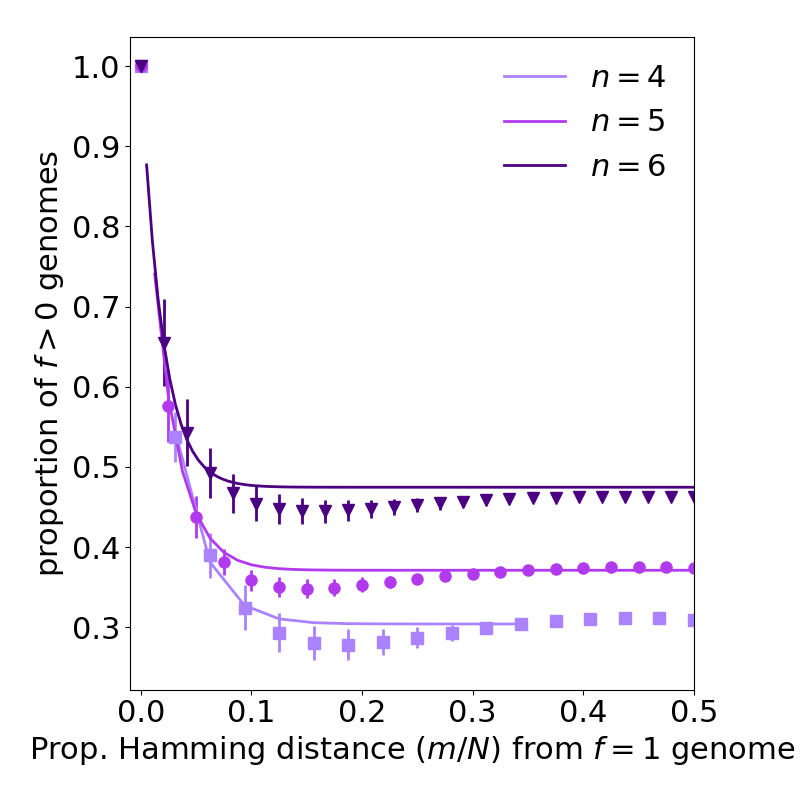
\includegraphics[width=0.7\textwidth,clip=true,trim=0cm 0cm 0cm 0cm]{../simsj/plot/smooth_fit_ff4.png}
\caption{\emph{A smooth fitness landscape.} The average proportion of
  genomes with non-zero fitness, accounting for all genomes at a
  Hamming distance of $m$ mutations away from a sample of ten
  maximally fit genomes is shown for networks of $n=4$ genes (squares
  indicate means, and error bars indicate standard error of the mean
  across fitness peaks), for networks of $n=5$ genes (circles) and
  $n=6$ genes (triangles).}
\label{fig:smooth_fit}
\end{center}
\end{figure}
\clearpage}

\afterpage{
\begin{figure}
\begin{center}
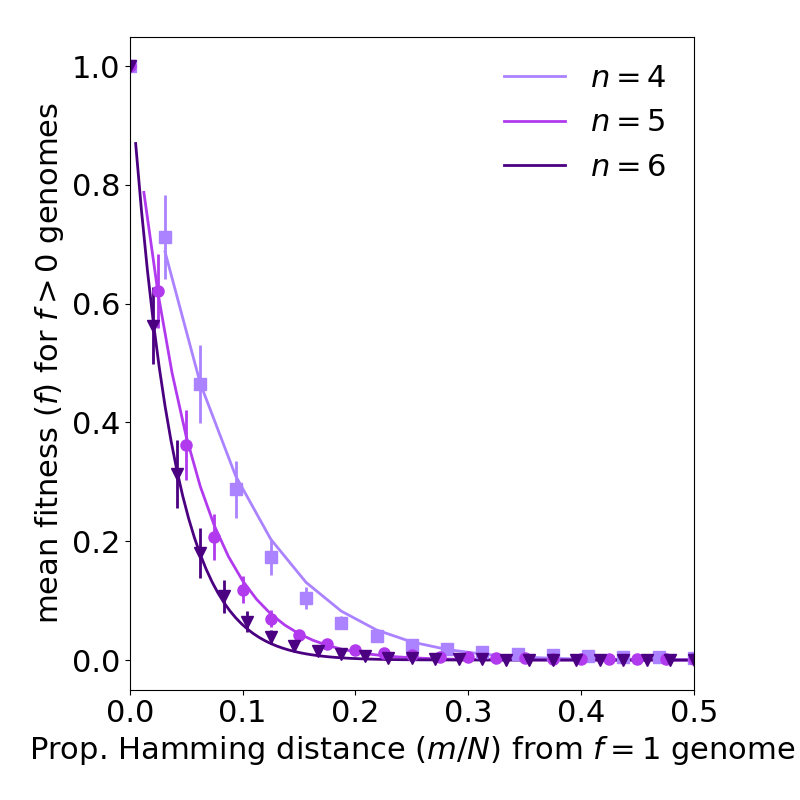
\includegraphics[width=0.7\textwidth,clip=true,trim=0cm 0cm 0cm 0cm]{../simsj/plot/fitness_increases_gradually_ff4.png}
\caption{\emph{Fitness increases monotonically towards the fitness
    peaks.} The average fitness of genomes with non-zero fitness
  decreases exponentially with each mutation of the genome $m$. Thus,
  once evolution has entered the vicinity of a fitness peak by
  un-directed search, a monotonically increasing gradient is available
  to guide evolution directly to the maximally fit configuration of
  the genome. A good fit to the function $h(m,k)$, plotted as solid
  curves, suggests that the smoothness of the fitness landscape
  reflects that genomes with non-zero fitness comprise a certain set
  of boolean interactions that are specified by a constant
  number of binary variables ($k\approx 10$, $k\approx 17$ and
  $k\approx 25$ for $n=4$, $n=5$ and $n=6$, respectively).}
\label{fig:fitness_increases}
\end{center}
\end{figure}
\clearpage}


\afterpage{
\begin{figure}
\begin{center}
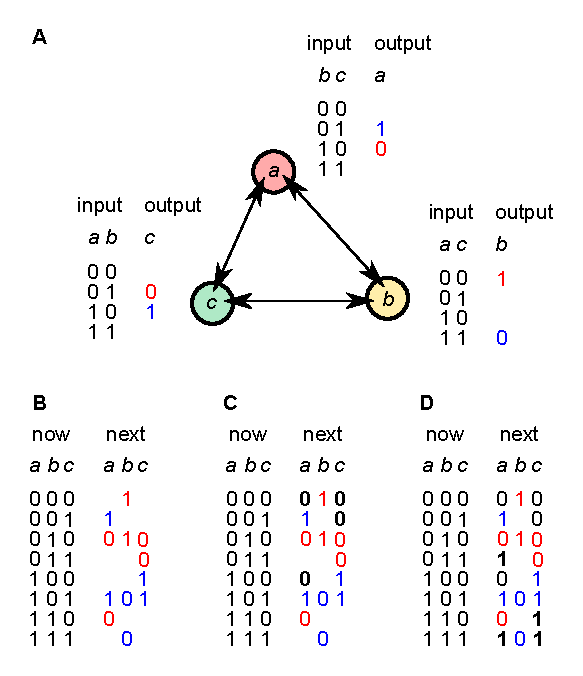
\includegraphics[width=0.7\textwidth,clip=true,trim=0cm 0cm 0cm 0cm]{Figures/S2.pdf}
\caption{\emph{Supplementary Figure S2: Networks of $n=3$ genes cannot
    map states 100 and 000 to point attractor states 101 and 010.}
  \textbf{A} Consider that in maximally fit networks, the anterior
  target state $101$ must transition next to state $101$ again. Thus
  for any solution, expression levels of 0 and 1 in genes $b$ and $c$
  must lead next to an expression level of 1 in gene $a$, levels $a=1$
  and $c=1$ must lead next to $b=0$ and levels $a=1$ and $b=0$ must
  lead next to $c=1$, thereby fixing three binary variables in the
  genome of any solution (blue). Three other variables are fixed by
  the constraint that the posterior target state $010$ must also
  transition into itself (red). \textbf{B} Fixing this motif of $2n=6$
  variables accordingly, determines that state $010$ can only be
  reached directly from states $000$, $011$, and $110$, and likewise
  that the target state $101$ can only be reached directly by states
  $001$, $100$, and $111$. \textbf{C} Linking any one of these states
  directly to its reachable target state makes the other target
  reachable from only the orthogonal state (e.g., a genome that
  transitions to $010$ from $000$ can only transition to state $101$
  from state $111$). \textbf{D} However, specifying any of these three
  possibilities makes those two states (e.g., $000$ and $111$)
  unreachable from any other, hence it follows that both initial
  states cannot reach their corresponding target states in any $n=3$
  network.}
\label{fig:supp2}
\end{center}
\end{figure}
\clearpage}

\afterpage{
\begin{figure}
\begin{center}
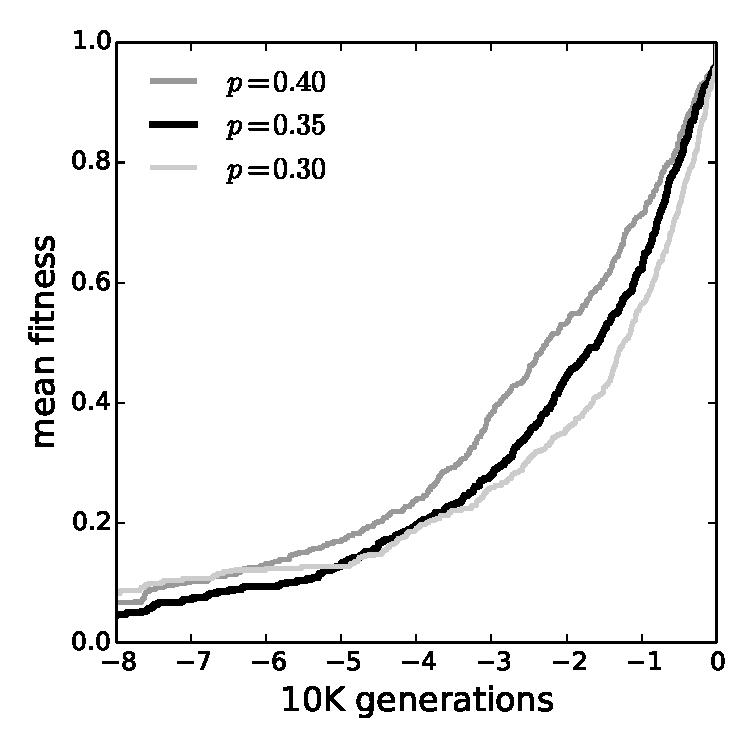
\includegraphics[width=0.7\textwidth,clip=true,trim=0cm 0cm 0cm 0cm]{Figures/S3.pdf}
\caption{\emph{Supplementary Figure S3}. At each of three mutation
  rates $p=0.30$, $p=0.35$ and $p=0.4$ the fitnesses in the
  generations proceeding the discovery of maximally fit genomes were
  averaged across all successful trajectories discovered within ten
  million generations. The resulting smooth plots reveal that
  incremental ascent of the fitness landscape in this model is
  possible. By comparison, un-directed search for fit genomes is a
  `needle-in-a-haystack' problem where peaks in the fitness landscape
  are sparse and isolated. Although no individual evolutionary
  simulation proceeds by incrementing fitness in such a continuous
  manner (see Figure 3), this visualisation clearly indicates that the
  progression towards peak fitness is incremental, and that the
  increment varies systematically with the free parameter of the model
  ($p$).}
\label{fig:supp3}
\end{center}
\end{figure}
\clearpage}



\section*{Figure Legends}

\noindent\textbf{Fig.\,1. The title for Figure 1}. Paste caption for Figure 1 here when finished.
\vspace{1em}\\

\noindent\textbf{Fig.\,2. The title for Figure 2}. Paste caption for Figure 2 here when finished.
\vspace{1em}\\

\noindent\textbf{Fig.\,3. The title for Figure 3}. Paste caption for Figure 3 here when finished.
\vspace{1em}\\

\noindent\textbf{Fig.\,4. The title for Figure 4}. Paste caption for Figure 4 here when finished.
\vspace{1em}\\

\noindent\textbf{Fig.\,5. The title for Figure 5}. Paste caption for Figure 5 here when finished.
\vspace{1em}\\

\noindent\textbf{Fig.\,6. The title for Figure 6}. Paste caption for Figure 6 here when finished.
\vspace{1em}\\


\section*{Supporting Information}

\noindent\textbf{S1 Code.} Source code required to reproduce the data presented in Figures 2--4 from the main text. From the command line, compile using e.g., `g++ -o model Wilson2018.cpp' and then run using e.g., `./model 0 5 0.35', where the parameters specify a random seed, the number of genes $n$, and the mutation rate $p$, respectively. Using a random seed less than 1 will use the current time as a seed. The program runs until a maximally fit genome is discovered and then prints the resulting genome configuration and a description of the corresponding attractor landscape.\\

%Contains i) %a standalone python script for recreating Fig.\,1, ii) an efficient c++ implementation of the evolutionary algorithm using the Monte Carlo huddling model for generating the data from which Figs.\,2-4 can be recreated, and iii) an efficient c++ implementation of the evolutionary algorithm using the agent-based huddling model for generating the data from which Figs.\,5-7 can be recreated. Please consult the README.txt files first for instructions about building, running, and analysing the models.

\noindent\textbf{Supplementary Figure S2. The title for Figure S2}. Paste caption for Figure S2 here when finished.
\vspace{1em}\\

\noindent\textbf{Supplementary Figure S3. The title for Figure S3}. Paste caption for Figure S3 here when finished.
\vspace{1em}\\


\end{document}


%NOTES FROM PREVIOUS DRAFTS











%%%%%%%%% FIRST FULL RESULTS INCLUDING F1 and F2

\section*{Results}

All figures in this paper can be recreated using the source code available in the supplementary materials as \emph{S1 Code}.

\subsection*{A `needle in a haystack' problem}

The goal is to characterise the fitness landscape in which gene interaction networks have been discovered, that from an initial differential expression of one gene (Fgf8) in the anterior of the forebrain, end with a specific set of (binary) stable expression gradients from anterior to posterior and vice versa. We must first establish the baseline rate at which such networks would be expected to be discovered by chance, i.e., the proportion of genomes that specify maximally fit networks.

It is instructive to first consider a simple network of $n=3$ genes. The binary genome space comprises $2^N=4,096$ networks (where $N=n2^{n-1}$), and for $n=3$, the problem can be formulated as one in which initial states $100$ and $000$ lead to corresponding states $101$ and $010$ as the only states occupying the limit cycles of two distinct attractors. An exhaustive search reveals that no genomes lead from initial states $100$ and $000$ to states $101$ and $010$ as the only states occupying the limit cycles of two distinct attractors. Thus, for a $n=3$ gene network, the problem is impossible.

Next we consider a $n=4$ gene networks and the corresponding genome space which comprises $2^{32}=4,294,967,296$ possible genomes. In this case the problem is to find networks where the initial posterior state $1000$ and the initial anterior state $0000$ leads to the corresponding final states $1010$ and $0101$. Knowing that in such networks iterating the target states $1010$ and $0101$ must transition directly to those same two states again allows binary states at $8/32$ loci in the genome to be set, and thus the genome space can be exhaustively searched by mapping out the attractor landscapes of only $2^{24}=16,777,216$ candidate networks. An exhaustive search of this genome space identified $475,122$ successful networks, i.e., 0.011\%.

For $n=5$ genes there are $2^{80}$ possible networks.The goal is to find initial networks where initial states 16 ($10000$) and 0 ($00000$) lead to the corresponding final states 21 ($10101$) and 10 ($01010$) as the only states occupying the limit cycle of separate attractors. Knowing that iterating the target states $10101$ and $01010$ must lead directly to those two states again allows binary states at $10/80$ locations to be set, and thus for the attractor landscapes of only $2^{70}$ networks to be mapped out by iterating their dynamics. Nonetheless an exhaustive search is not feasible. Instead we randomly generated $2^{32}$ random networks (for comparison with the $n=4$ case), and discovered $59,088$ maximally fit networks, i.e., 0.0014\%. Therefore, we estimate that the baseline rate at which maximally fit networks should be discovered by blind search for a $n=5$ gene network is between 1 and 2 in every $100,0000$ generations.

Together these simulation results indicate that the problem of developing complementary gene expression patterns may be solved for networks comprising a minimum of $n=4$ genes, and that the problem increases in difficulty as the number of interacting genes increases.

Figure 2 shows the attractor landscape in a maximally fit network of $n=5$ interacting genes.

\subsection*{Smoothing the fitness landscape}

Next we ask whether the discovery of maximally fit networks may be accelerated by natural selection under a fitness function designed to exploit a potential relationship between the structure of the genome space and the laws by which attractors self-organise in the network dynamics. Instead of searching the genome space randomly, we can modify our definition of fitness to also favour genomes that do not necessarily specify maximally fit networks, but which display some of the properties of fit networks. To this end, we define all genomes that specify networks in which the initial anterior and posterior states do not belong to different point attractors as having zero fitness ($f=0$). For the remaining genomes, we measure the Hamming distance of the single state occupying the limit cycle of the attractor that comprises the posterior state 16 from the posterior target state 21 as $h_p$ and the distance of the single state occupying the limit cycle of the attractor that comprises the anterior state 0 from the posterior target state 10 as $h_a$, and define,

\begin{equation}
f=1-\alpha(h_p+h_a),
\end{equation}

\noindent where $\alpha$ specifies a small (arbitrary) cost to final (stable) gene expression patterns that increases with the deviation of these patterns from the target pattern, and which selection may thus optimise. The rationale is that a gene interaction network that transitions into final states more similar to the full set of complementary expression gradients, while not maximally fit, may nonetheless result in some developmental functionality. This definition of fitness need not be biologically valid in order for the resulting evolutionary results to be informative, but we note that it satisfies the condition that no direct transmission of information about the state of the phenotype. We refer to this fitness function as \emph{F1}. To simulate evolution in this model, we maintain a single genome, and in each generation flip all bits in the genome with probability $p\in\{0,0.5\}$, and accept the new genome if the fitness of the resulting network is increased as a result.

The resulting evolutionary dynamics are shown in Figure XX ($\alpha=0.1$). An initial genome was randomly generated upon discovery of a maximally fit genome ($f=1$), and a total of X generations were iterated in each simulation in order to estimate the statistics. For simulations run independently for a range of mutation rates, the rate at which maximally fit networks was discovered was substantially greater than the baseline discovery rate: X for $p=0.X$, Y for $p=0.Y$, and Z for $p=0.Z$. Thus, selecting for point attractors with states at the limit cycle that are closer (smaller Hamming distance) from the target states reveals a smoothness to the distribution of fit genomes in genome space that can be exploited to accelerate their discovery by natural selection.

Figure Z shows the distribution of discovery rates for each mutation rate on a logarithmic scale. In addition to demonstrating that the `needle in a haystack' fitness landscape may be smoothed, these evolutionary dynamics indicate that maximally fit genomes are distributed in the genomes space according to some characteristic distance, as indicated by a consistent peak in the distribution of discovery rates in Figure Z at approximately Z generations for each mutation rate.

These results together confirm the hypothesis that a relationship between the structure of the genome space and the laws by which attractors self-organise in the network dynamics exists, and that it can be exploited to accelerate the evolutionary search for gene-interaction networks from which complementary gene expression patterns emerge, without direct transmission of information from phenotype to genotype.

\subsection*{Self-organised criticality in the evolution of cortical development}

To further establish how structure in the distribution of maximally fit networks may be exploited, we next relax the selection pressure further to also favour networks which from the correct initial conditions satisfy the target configuration in the anterior and posterior locations \emph{at some stage} during the attractor dynamics. Specifically, if conditions ii, iii, and iv are met, and $d(s)$ is the distance of state $s$ from the limit cycle, then the fitness of the genome $f$ is defined according to fitness function F2, as,

\begin{equation*}
f=1-\left(d(10)+d(21)\right)/2^{n+1},
\end{equation*}

\noindent or else $f=0$. Again we maintain a single genome, and in each generation flip all bits in the genome with probability $p\in\{0,0.5\}$, and accept the new genome if the fitness of the resulting network is increased as a result.

In contrast to the relatively smooth increment in fitness under fitness function F1, the evolution under fitness function F2 reveals a dynamics more akin to `punctuated equilibria', in which increasingly long periods of stasis are punctuated by increments in fitness. The corresponding plot of discovery rates in Figure Y reveals an approximately power law distribution.

Thus relaxing the selection pressure (in F2) that only point attractors have non-zero fitness (as in F1), reveals that the distribution of fit genomes has a scale-free, self-similar geometry. Under F2, the rate at which maximally fit networks are discovered is further increased (compared to F1): X for $p=0.X$, Y for $p=0.Y$, and Z for $p=0.Z$. Hence this self-similar geometry may be exploited to further accelerate the discovery of maximally fit networks by natural selection.

Moreover, the power law distribution of discovery rates revealed by evolution under F2 is robust to the only free parameter of the model, the mutation rate $p$. This is a strong indicator of self-organised criticality in the underlying evolutionary dynamics.

Furthermore the exponent of the power law fit at each mutation rate indicates that the underlying dimensionality is non-integer, suggesting that the underlying geometry of the fitness landscape under fitness F2 is fractal.

\subsection*{Extra notes}

In our model $k=n-1$ is the number of genes to which each is connected. It has been shown that if $p$ is the proportion of the $N$ truth table entries that specify an output of 0 (no gene expression at the next iteration), then $k_c=(2p(1-p))^{-1}$ is a critical value such that when $k_c<k$ the network dynamics will be unstable, insofar as from two nearby states (small Hamming distance) the dynamics will diverge and the Hamming distance will increase. In the present model we are interested in precisely such networks, insofar as two initial states separated by the minimal Hamming distance of 1 should lead to two target states separated by a maximal Hamming distance of $n$. Thus it follows that for maximally fit networks, $p > \frac{1}{2}\left(1-\sqrt{1-\frac{2}{k}}\right)$. For networks of $n=5$ genes $k_c<k$ when $p>0.14644661$ and hence at least 12 of the 80 binary variables that specify the genome are 0.

\serction*{Discussion}

To summarise, the main results are as follows 1) a minimum of four interacting genes is required to specify network dynamics from which complementary gradients emerge; 2) the evolution of gene-network interactions for $n=5$ genes is a `needle in a haystack’ problem, and for $n>3$, the problem increases; 3) selecting for point attractors with states at the limit cycle that are closer (smaller Hamming distance) from the target states reveals a smoothness to the distribution of fit genomes in genome space that can be exploited to accelerate their discovery by natural selection; 4) Specifically, fit genomes are distributed in the genomes space according to some characteristic distance, as indicated by a peak in the distribution of discovery rates by evolving under this fitness function; 5) relaxing the selection pressure that only point attractors have non-zero fitness reveals an evolutionary dynamics that resembles punctuated equilibria, and a distribution of fit genomes that has a scale-free, self-similar geometry that may be exploited to further accelerate their discovery by natural selection. This is evidenced by the emergence of a power law distribution in the discovery rate; 6) The power law distribution of discovery rates under F2 is robust to the free parameter of the model, the mutation rate $p$, which is a hallmark of self-organised criticality; 7) A non-integer dimension obtained from power law fits to the distribution of discovery rates suggest that the underlying geometry of the fitness landscape under F2 may be fractal.


\begin{itemize}
\item important to acknowledge that cortical space is very crudely divided into two compartments and more might be more appropriate
\item also important to note that the two compartments are assumed not be coupled. You could imagine having a network in which the state of the expression level in one compartment is simply not the state of the expression level in the other.
\item should point out that different choices of $K$ are possible, including $K=N$, i.e., where genes are also influencing themselves, but that a gene turning itself on can be achieved by including extra steps of the dynamics, and that `no connection' is possible (i.e., by completing the truth table with the same output irrespective of the state of the value of that particular connection).
\item also important to note that the expression levels do not necessarily persist indefinitely in the final cortex.
\item Also important to note that we have note evaluated whether the two initial states should be the same distance from the limit cycle - not sure if it matters.
\item Is there something more to be made of the problem here in its general form, i.e., taking one bit of information (Fgf8 expression level) and turning it into 5 bits of information? What is happening to information in this system?
\item perhaps we can get a handle on this by considering in more formal terms why the problem cannot be solved by three genes?
\item note that Jim and I found a Baldwin-esque boolean nets paper before, where trying two steps ahead accelerated evolution.
\item must discuss Deacon's statement that Baldwin effect can be without learning.
\item note that networks favoured by our relaxed fitness function do not necessarily occupy the target state in the anterior and posterior region at the same time, and that imposing this.
\end{itemize}



%%%%%%%%% RESULTS DRAFT FROM EARLIER
\section*{Results}


\subsection*{Emergence of punctuated equilibria}

If we evolve the model by flipping the binary state of each bit in the genome with a probability of 0.3, and accept such changes only if they improve fitness, and when fitness is maximal reset to a new entirely random genome, then 0.00337\% networks are successful.

The evolution of ten simulations are shown. According to the fitness function (Equation X), a genome has non-zero fitness if proceeding from the initial states 10000 and 00000 at some point reaches states 10101 and 01010 respectively on different attractors, and fitness is greater if the distance of each target state from the limit cycle is reduced. Traces are aligned so that the generations at which maximally fit genomes (fitness = 1) are first discovered are plotted at generation zero on the right hand side. Evolution in each case proceeds from left to right. The characteristic shape of each trace indicates that evolution in this model is predicted to proceed via long periods of stasis that are punctuated by sharp increases in fitness. Thus the evolutionary dynamics predicted by this model may be described as `punctuated equilibria'. The trace highlighted with a thicker line shows the evolution of the maximally fit network whose developmental interactions are represented in Figure 2.

\subsection*{Self-organized criticality}

The evolution of networks was continued for a total of 10,000,000 generations. Each time a maximally fit network was discovered the initial conditions were randomised and the number of generations between the discovery of maximally fit networks was recorded. The process was repeated for mutation rates of $p=0.3$, $p=0.35$, and $p=0.40$, and in each case the distribution was well approximated by a straight line on a logarithmic plot, indicating a power law distribution. The slope of the power law fit was similar over the range of mutation rates shown, indicating a robustness to the free parameters of the system (in this case the mutation rate $p$), which is a hallmark of criticality.

\subsection*{The Baldwin Effect}

At each of three mutation rates $p=0.30$, $p=0.35$ and $p=0.4$ the fitnesses in the generations proceeding the discovery of maximally fit genomes were averaged across all successful trajectories discovered within ten million generations. The resulting smooth plots reveal that incremental ascent of the fitness landscape in this model is possible. By comparison, un-directed search for fit genomes is a `needle-in-a-haystack' problem where peaks in the fitness landscape are sparse and isolated. No individual evolutionary simulation proceeds via a continuous increment in fitness, this visualisation clearly indicates that the progression towards peak fitness is incremental, and that the increment varies systematically with the free parameter of the model ($p$).


%Figure 6 confirms that the proportion of networks with non-zero fitness (i.e., those in which the initial and complementary mature expression patterns correctly occupy distinct attractors) decreases exponentially with each mutation. Specifically, if $x$ is the number of mutations and $y(x)$ is the proportion of mutated genomes yielding non-zero fitness, then the relationship is given by,

%\begin{equation*}
%y(x)=\alpha 2^{-\beta x}.
%\end{equation*}

%For $n=4$ networks, all genomes up to five mutations from genomes specifying maximally fit networks could be evaluated in reasonable compute time, and a fit by linear regression to the averages obtained with respect to ten fitness peaks yielded  estimates of $\beta=0.76$ and $\alpha=0.90$. For $n=5$ networks, all genomes up to four mutations away were evaluated, yielding estimates of $\beta=0.55$ and $\alpha=0.96$.
